\subsection{普遍严格映射}

设

\[
\begin{array}{c} \mathrm {X^ {\prime}} \xrightarrow {f ^ {\prime}} \mathrm{X} \\ \Big \downarrow_ {p ^ {\prime}} \\ \mathrm {B^ {\prime}} \xrightarrow {f} \mathrm{B} \end{array}
\]

为一个笛卡尔方块，其中 p 是严格的。映射 \(p'\) 未必是严格的 (cf. 注 1)。然而，若 A 在 B 中是开的（相应地，闭的），则映射 \(p_A: \overline{p}^{1}(A) \to A\) 是严格的。

定义 6. --- 设 p: X → B 为一个映射。我们称 p 是普遍严格的，如果对每个笛卡尔方块

\pandocbounded{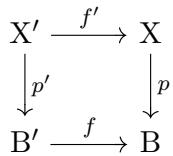
\includegraphics[keepaspectratio]{images/part001_50963eb1.jpg}}

映射 p' 是严格的。

普遍严格映射是严格的。采用定义 6 中的记号，若 \(p\) 是普遍严格的，则 \(p'\) 也是普遍严格的。这由定义立即得出。

推论. --- 开映射、逆紧映射以及具有连续局部截面的映射都是普遍严格的。

例. --- 设 B 为一个拓扑空间，\((\mathrm{A}_{i})_{i\in\mathrm{I}}\) 为 B 的一个覆盖；用 A 表示族 \((\mathrm{A}_{i})_{i\in\mathrm{I}}\) 的和空间，用 \(p: A \to B\) 表示典型映射。在下列两个假设中的每一个之下，映射 p 都是普遍严格的：

\begin{enumerate}
\def\labelenumi{(\roman{enumi})}
\item
  对每个点 \(b \in B\) ，存在 \(i \in I\) ，使得 b 是 \(A_{i}\) 的一个内点；
\item
  族 \((A_{i})\) 是局部有限的，且诸 \(A_{i}\) 是 B 的闭子集。
\end{enumerate}

在假设 (i) 之下，映射 p 在每点的一个邻域内有连续截面。在假设 (ii) 之下，映射 p 按和空间的定义（相应地，由 TG, I, p. 6, prop. 4 与 TG, I, p. 75, th. 1）是逆紧的。因此它是普遍严格的。

注. --- 闭映射未必是普遍严格的 (cf. TG, I, p. 96, exerc. 6)。

命题 11. --- 设

\pandocbounded{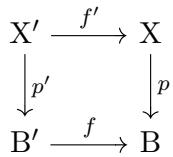
\includegraphics[keepaspectratio]{images/part001_02f1b349.jpg}}

为一个笛卡尔方块。

\begin{enumerate}
\def\labelenumi{\alph{enumi})}
\item
设 f 是严格且满射的。于是，若 p' 是开的（相应地，闭的；相应地，逆紧的），则 p 亦然。
\item
设 f 是闭且满射的。若 p' 是严格的，则 p 是严格的。
\item
设 f 是普遍严格的。若 p' 是普遍严格的，则 p 是普遍严格的。
\end{enumerate}

首先注意，对 X 的每个子集 A，我们有

\[
p ^ {\prime} ((\stackrel {- 1} {f ^ {\prime}}) (\mathrm{A})) = \stackrel {- 1} {f} (p (\mathrm{A})).\tag{20}
\]

事实上，若 \(x' \in (f')^{-1}(\mathrm{A})\) ，则 \(f(p'(x')) = p \circ f'(x') \in p(\mathrm{A})\) 。反之，若 \(b' \in f^{-1}(p(\mathrm{A}))\) ，设 \(x \in A\) 满足 \(f(b') = p(x)\) 。由笛卡尔方块的定义，存在唯一的 \(x' \in X'\) ，使得 \(f'(x') = x\) 且 \(p'(x') = b'\) ，从而 \(b' \in p'((f')^{-1}(\mathrm{A}))\) 。

设 f 是一个开映射且 \(p'\) 是一个严格映射。

集合 \((f')^{-1}(\mathrm{A})\) 在 \(\mathrm{X}'\) 中是开的（相应地，闭的）。于是集合 \(p'((f')^{-1}(\mathrm{A}))\) 在 \(\mathrm{B}'\) 中是开的（相应地，闭的）。由关系式 (20)，它对由 \(f\) 定义的等价关系也是饱和的。由于映射 \(f\) 假设为满射，我们有 \(p(\mathrm{A}) = f(p'((f')^{-1}(\mathrm{A})))\) ，又由于它是严格的，集合 \(p(\mathrm{A})\) 在 B 中是开的（相应地，闭的）。于是映射 \(p\) 是开的（相应地，闭的）。

为使一个连续映射是逆紧的，必须且只需它是闭的且它的纤维是拟紧的 (TG, I, p. 75, th. 1)。若映射 \(p'\) 是逆紧的，则由前所证，映射 \(p\) 是闭的。我们来研究它的纤维：若 \(b \in B\) ，设 \(b' \in B'\) 满足 \(f(b') = b\) 。由 I, p. 10 的推论，映射 \(f'\) 诱导出一个同胚 \(X_{b'}' \to X_b\) 。由于 \(p'\) 是逆紧的，\(X_{b'}'\) 是拟紧的，从而 \(X_b\) 也是。于是映射 \(p\) 是逆紧的。

我们来证明 b) 与 c)。令 \(Y = p(X)\) ，\(Y' = p'(X')\) 。把关系式 (20) 应用于 X，就得到 \(Y' = f^{-1}(Y)\) 。用 g 表示由 f 诱导的从 \(Y'\) 到 Y 中的映射。在情形 b)，由 I, p. 18 的注 1，映射 g 是严格的。在情形 c)，由定义 6 它是严格的，因为方块

\pandocbounded{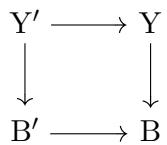
\includegraphics[keepaspectratio]{images/part001_f35053b2.jpg}}

是笛卡尔的。

用 \(q\) 与 \(q'\) 分别表示从 X 到 Y 以及从 \(X'\) 到 \(Y'\) 中的映射，它们由映射 \(p\) 与 \(p'\) 诱导。

\[
\begin{array}{c} \mathrm {X^ {\prime}} \xrightarrow {f ^ {\prime}} \mathrm{X} \\ \Big \downarrow q ^ {\prime} \\ \mathrm {Y^ {\prime}} \xrightarrow {g} \mathrm{Y} \end{array}
\]

由于 \(f\) 是满射，\(f'\) 也是满射；由命题 9 b)，\(p\) 是严格的。

推论 1. --- 设映射 f 是普遍严格且满射的，且映射 p' 是普遍严格的。则映射 p 是普遍严格的。

设

\[
\begin{array}{c} \mathrm{Y} \xrightarrow {g ^ {\prime}} \mathrm{X} \\ \Biggl \downarrow q \\ \mathrm{C} \xrightarrow {g} \mathrm{B} \end{array}
\]

为一个笛卡尔方块；目标是证明映射 q 是严格的。由 I, p. 16 的注 3，方块

\[
\begin{array}{c} \mathrm {X^ {\prime}} \times_ {\mathrm{X}} \mathrm{Y} \xrightarrow {\mathrm{pr} _ {1}} \mathrm {X^ {\prime}} \\ \Biggl \downarrow r \\ \mathrm {B^ {\prime}} \times_ {\mathrm{B}} \mathrm{C} \xrightarrow {\mathrm{pr} _ {1}} \mathrm {B^ {\prime}} \end{array}
\]

和

\[
\begin{array}{c} \mathrm {X^ {\prime} \times_ {X} Y\xrightarrow {pr_ {2}} Y} \\ \Big \downarrow r \\ \mathrm {B^ {\prime} \times_ {B} C\xrightarrow {pr_ {2}} C} \end{array}\tag{21}
\]

都是笛卡尔的，其中 \(r \colon X' \times_{X} Y \to B' \times_{B} C\) 表示由 \((p', q)\) 诱导的映射。由于映射 \(f\) 是普遍严格且满射的，映射 \(\mathrm{pr}_2 \colon B' \times_{B} C \to C\) 亦然 (I, p. 20, def. 6 与 I, p. 10, prop. 4 的推论)。另一方面，映射 \(r\) 是严格的，因为 \(p'\) 假设为普遍严格的。把命题 11 c) 应用于笛卡尔方块 (21)，映射 \(q\) 是严格的。

推论 2. --- 设 B 与 X 为拓扑空间，\(p\colon X \to B\) 为一个连续映射。设 \((A_i)_{i \in I}\) 为 B 的一族子集，它构成 B 的一个开覆盖，或者构成 B 的一个局部有限的闭覆盖。若对每个 \(i \in I\) ，映射 \(p_{A_i}\colon \overline{p}^1(A_i) \to A_i\) 都是严格的（相应地，普遍严格的），则映射 p 是严格的（相应地，普遍严格的）。

对每个 \(i \in \mathrm{I}\) ，令 \(\mathrm{Y}_i = \overline{p}^{1}(\mathrm{A}_i)\) ，\(p_i = p_{\mathrm{A}_i}\) 。设 A 为族 \((\mathrm{A}_i)_{i \in \mathrm{I}}\) 的和空间，Y 为族 \((\mathrm{Y}_i)_{i \in \mathrm{I}}\) 的和空间；用 \(f: \mathrm{A} \to \mathrm{B}\) （相应地，\(g: \mathrm{Y} \to \mathrm{X}\) ，\(q: \mathrm{Y} \to \mathrm{A}\) ）表示由典型单射的族 \(A_i \rightarrow B\) （相应地，典型单射的族 \(Y_i \rightarrow X\) 与诸映射 \(p_i\) ）诱导的映射。方块

\[
\begin{array}{c} \mathrm{Y} \xrightarrow {g} \mathrm{X} \\ \Big \downarrow q \\ \mathrm{A} \xrightarrow {f} \mathrm{B} \end{array}
\]

是一个笛卡尔方块 (例, I, p. 10 与 p. 14)。由 I, p. 20 的推论，映射 \(f\) 是普遍严格的。于是由命题 11，只需证明映射 \(q\) 是严格的（相应地，普遍严格的），如果诸映射 \(p_i\) （\(i \in I\) ）是严格的（相应地，普遍严格的）。这样我们就把该推论的证明化归为这样的情形：诸集合 \(A_i\) （\(i \in I\) ）构成空间 B 的一个由既开又闭的部分组成的分拆，以下即作此假设。

设诸映射 \(p_i\) （\(i \in I\) ）中的每一个都是严格的。若 U 是 X 的一个开子集，且对由 p 定义的等价关系是饱和的，则集合 \(p_i(\mathrm{X}_i \cap \mathrm{U})\) 在 \(\mathrm{A}_i\) 中是开的，从而 \(p(\mathrm{U}) = \bigcup_{i \in \mathrm{I}} p_i(\mathrm{X}_i \cap \mathrm{U})\) 在 B 中是开的。于是映射 p 是严格的。

现在设诸映射 \(p_{i}, i \in I\) 中的每一个都是普遍严格的，我们来证明映射 p 是普遍严格的。设 C 为一个拓扑空间，\(h: C \to B\) 为一个连续映射。目标是证明映射 \(pr_{1}: X \times_{B} C \to C\) 是严格的。空间 C 等同于族 \(C_{i} = h^{-1}(A_{i})\) 的和空间，而空间 \(X \times_{B} C\) 等同于族 \(X \times_{B} C_{i} = X_{i} \times_{A_{i}} C_{i}\) 的直和空间。由于 \(p_{i}\) 是普遍严格的，映射 \(pr_{1}: X_{i} \times_{A_{i}} C_{i} \to C_{i}\) 是严格的。由前所证，映射 \(pr_{1}: X \times_{B} C \to C\) 是严格的。这就证明了映射 p 是普遍严格的。

